\chapter{SAF microarchitecture taxonomy}
\label{chapter:saf_microarchitectures}

\section{SAF microarchitectures}
\label{chapter:saf_microarchitectures_section}

This section will overview the taxonomy of SAF microarchitectures considered in this work. SAF microarchitectures implement SAFs. Though not a requirement, in practice all SAF microarchitectures considered in this work were well-described as compound components, and conversely the only compound components modeled in this work happen to be SAF microarchitectures.

\subsection{Format microarchitectures}

\begin{figure}[H]
    \centering
    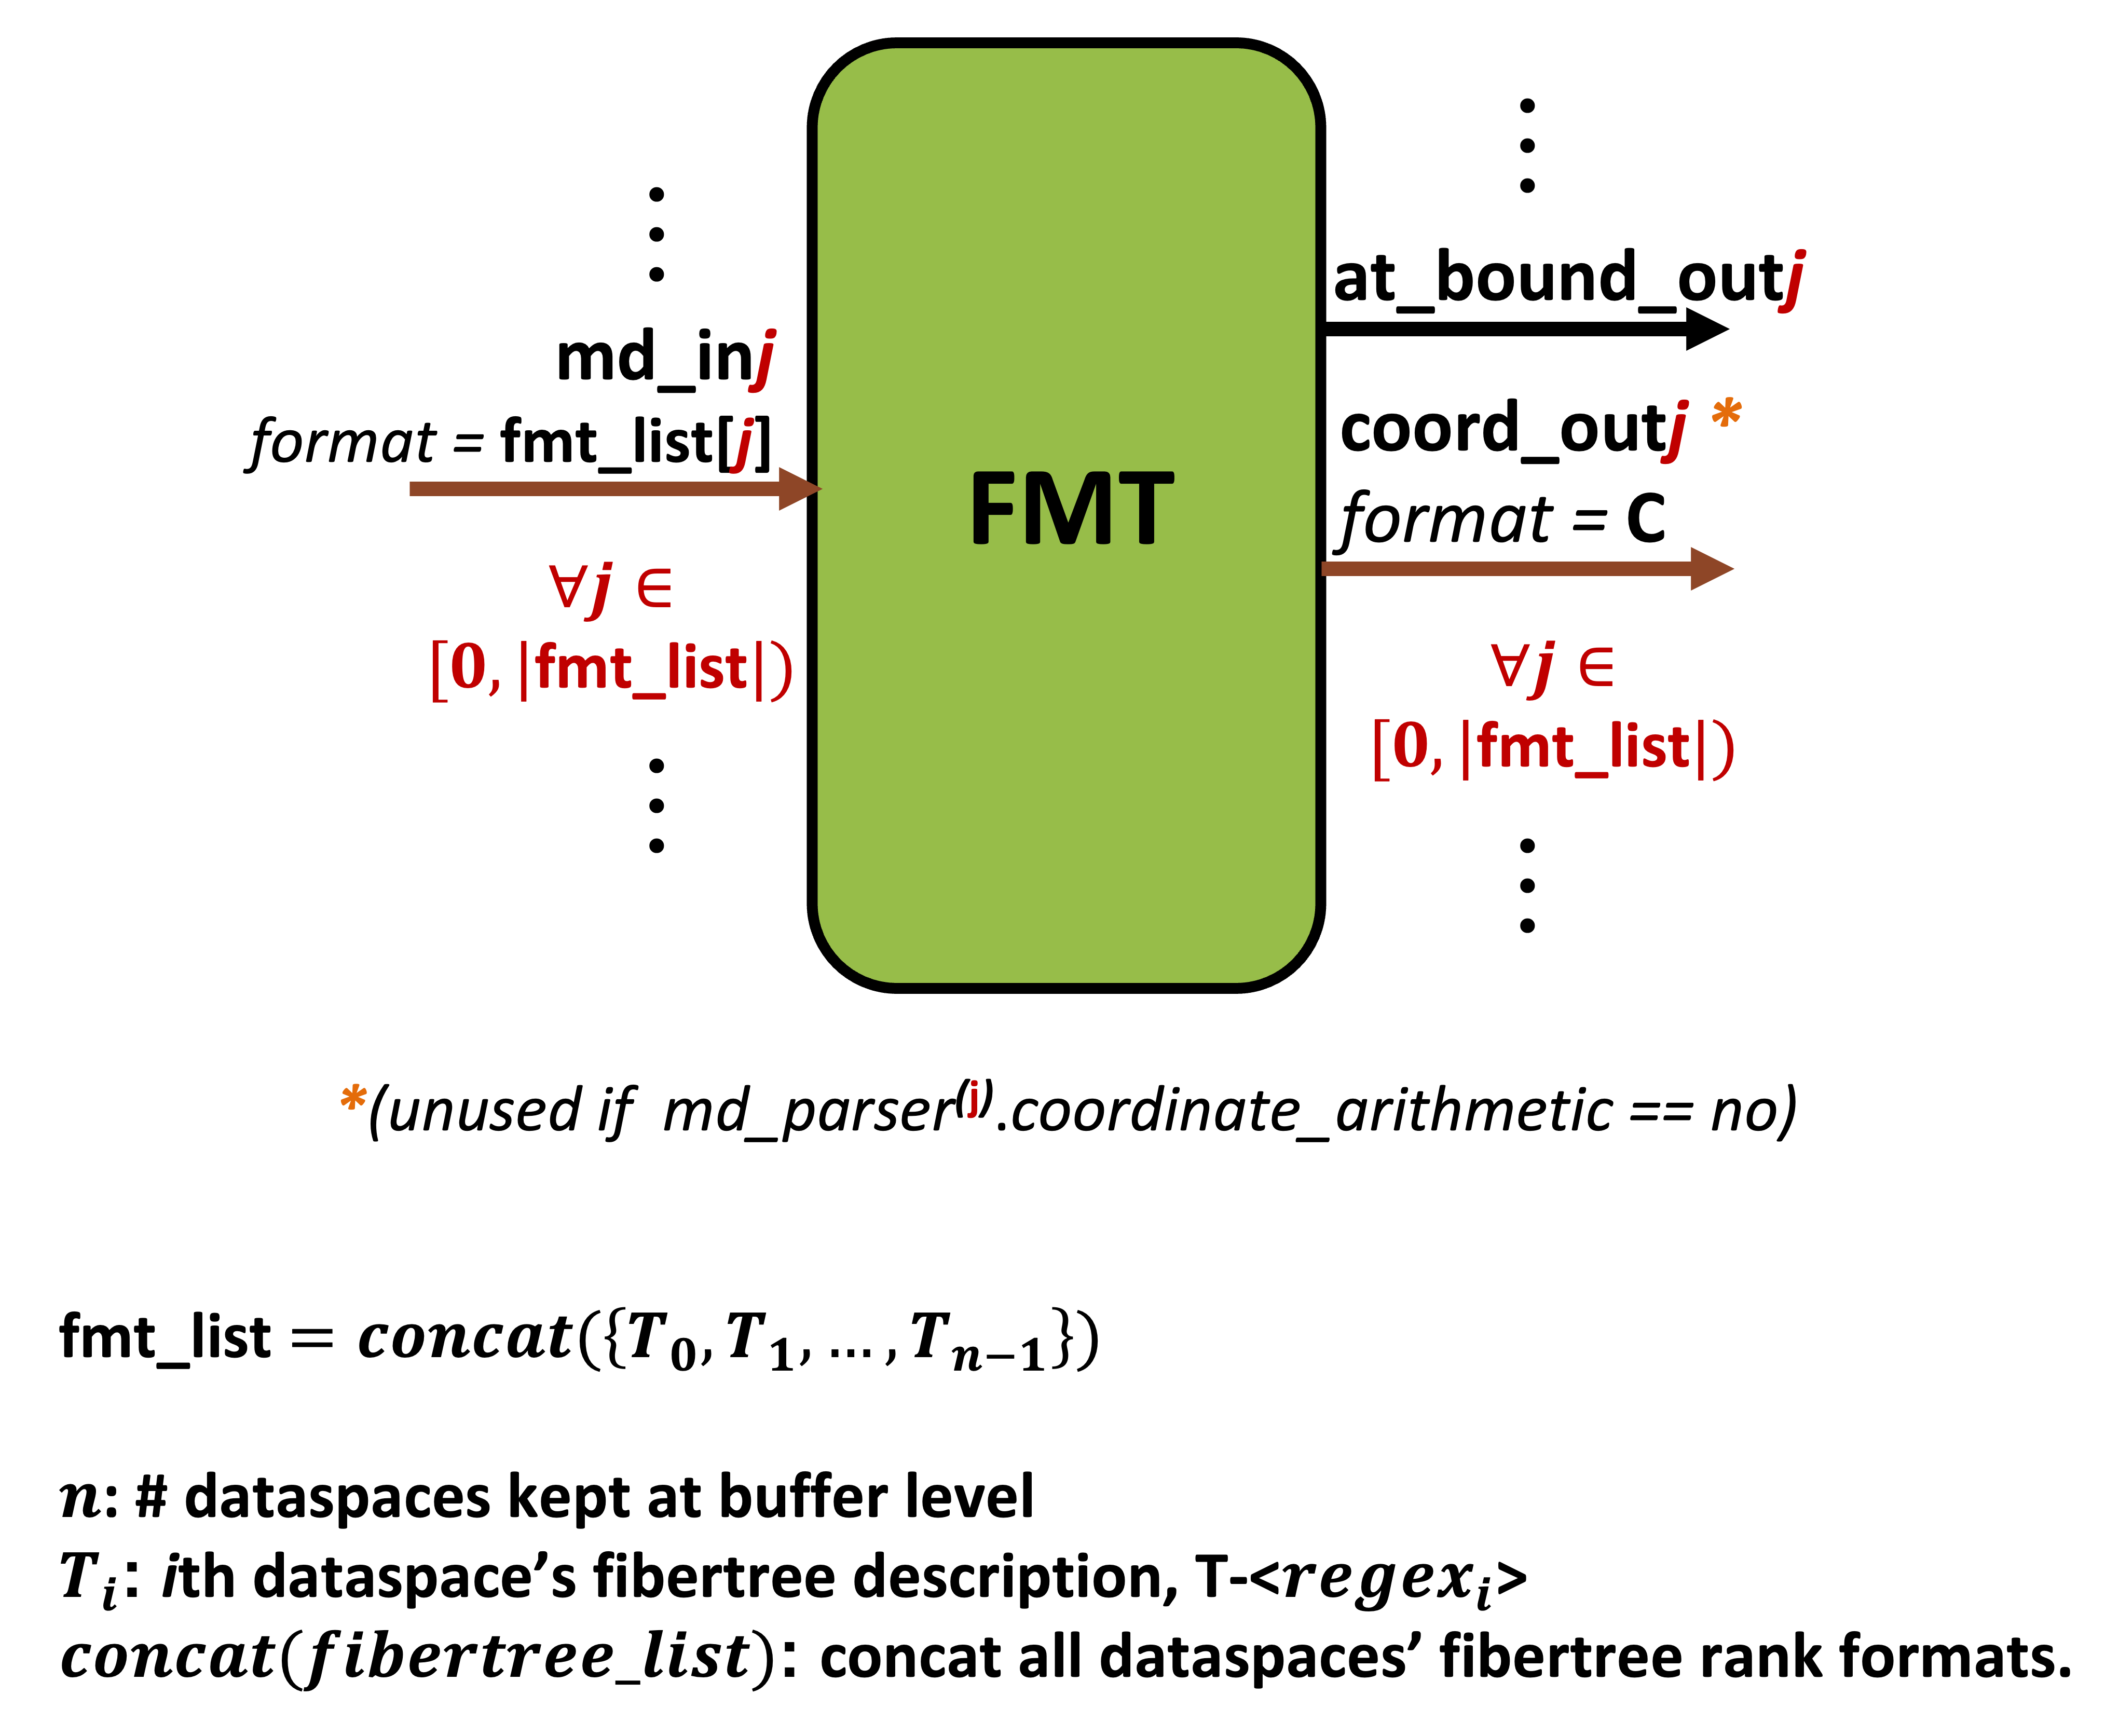
\includegraphics[width=0.95\textwidth]{figures/FMT.png}
    \caption{Format microarchitecture compound component template. If an architectural buffer has a format SAF, a format microarchitecture must be bound to it. The fmt\_list parameter expects a list of rank formats. The architectural buffer keeps\cite{timeloop} one or more dataspaces\cite{timeloop}, at least one of which exploits a format SAF. fmt\_list is assumed to have been derived from concatenating the fiber representation regexes\cite{szebook} for all kept dataspaces' fibertrees, excluding dataspaces which do not exploit a format SAF.}
    \label{fig:FMT}
\end{figure}

%\begin{table}[H]
%\centering
%\begin{tabular}{l}
%\toprule
% fibertree   \\
%\midrule
% *           \\
%\bottomrule
%\end{tabular}
%\caption{Specializations of format microarchitecture}
%\label{tab:format_microarchitecture_specializations}
%\end{table}

\begin{figure}[H]
    \centering
    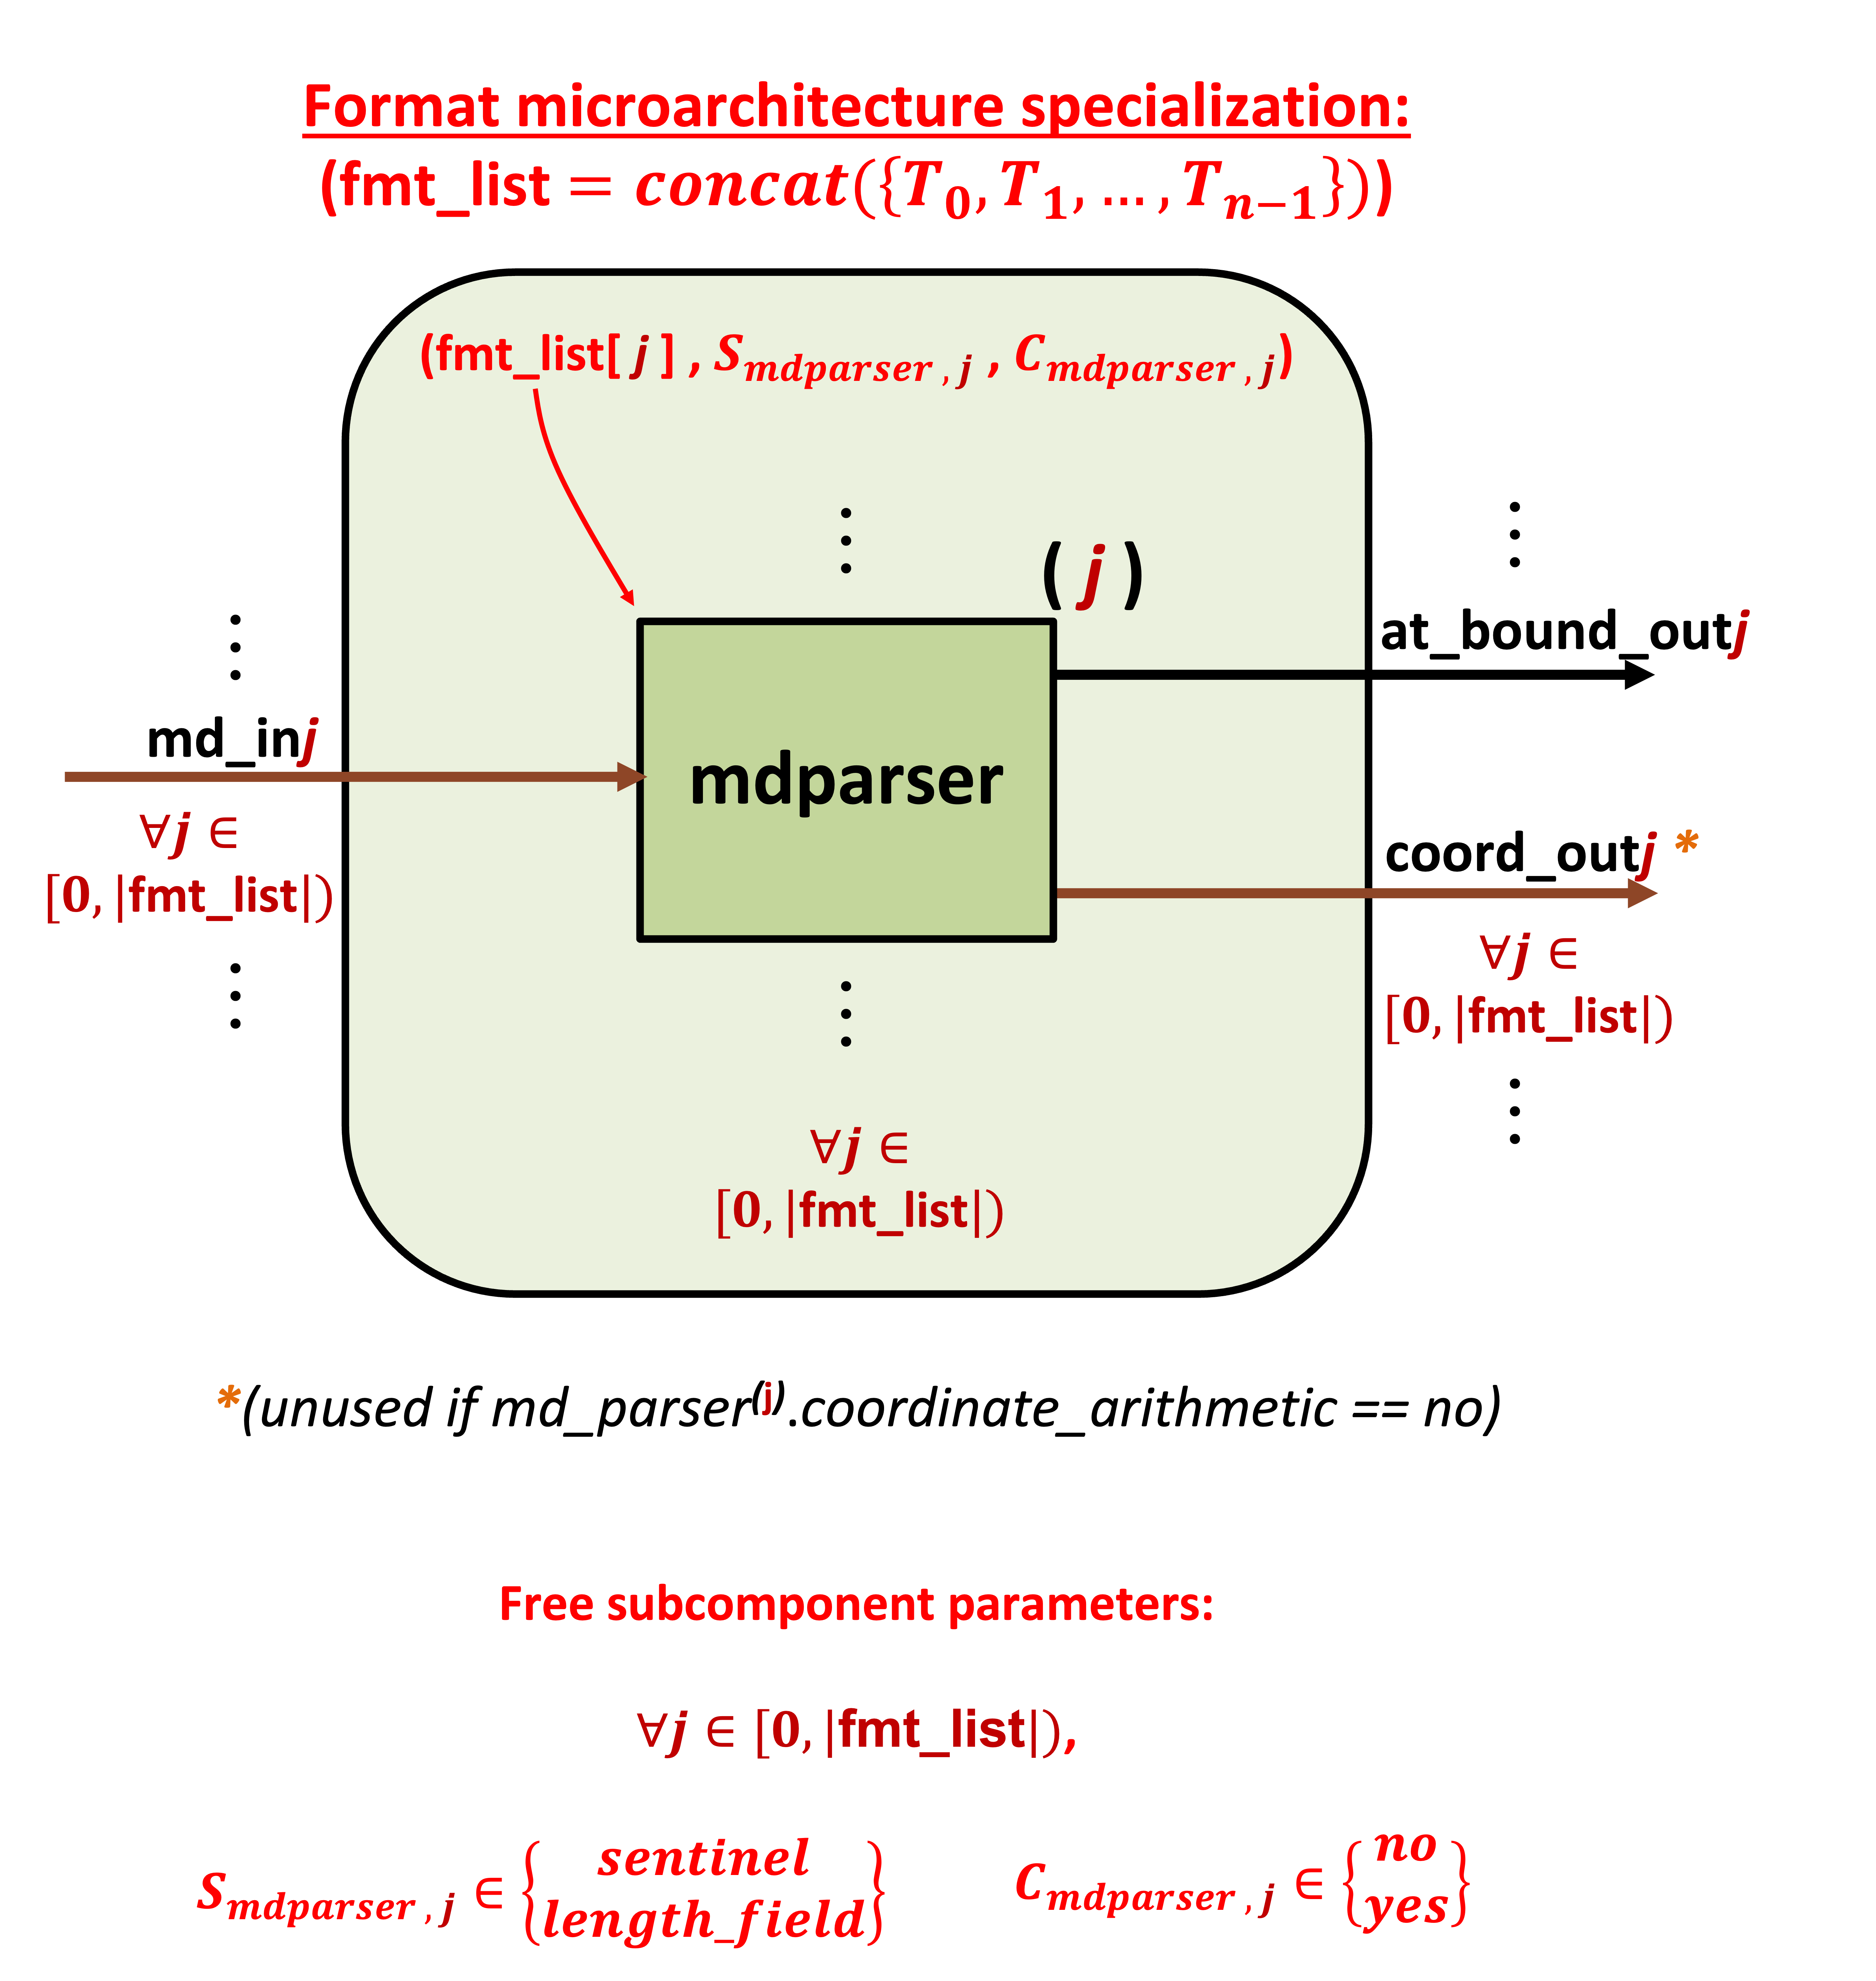
\includegraphics[width=0.95\textwidth]{figures/FMT_all.png}
    \caption{Format microarchitecture implementation topology. Every rank, in every fibertree, in every kept dataspace which is subject to a format SAF for a given buffer, has a corresponding metadata parser in the format microarchitecture topology. This implementation topology is universal for format microarchitectures regardless of the specific \textit{fmt\_list} parameter value. Each metadata parser subcomponent, however, has two free parameters. Setting \textit{coordinate\_arithmetic = no} for the $j$th metadata parser, means that that format microarchitecture will not support coordinate arithmetic for the corresponding fibertree rank. This can conserve resources i.e. if the rank is being contracted anyway.}
    \label{fig:FMT_all}
\end{figure}

\subsection{Skipping microarchitectures}

\begin{figure}[H]
    \centering
    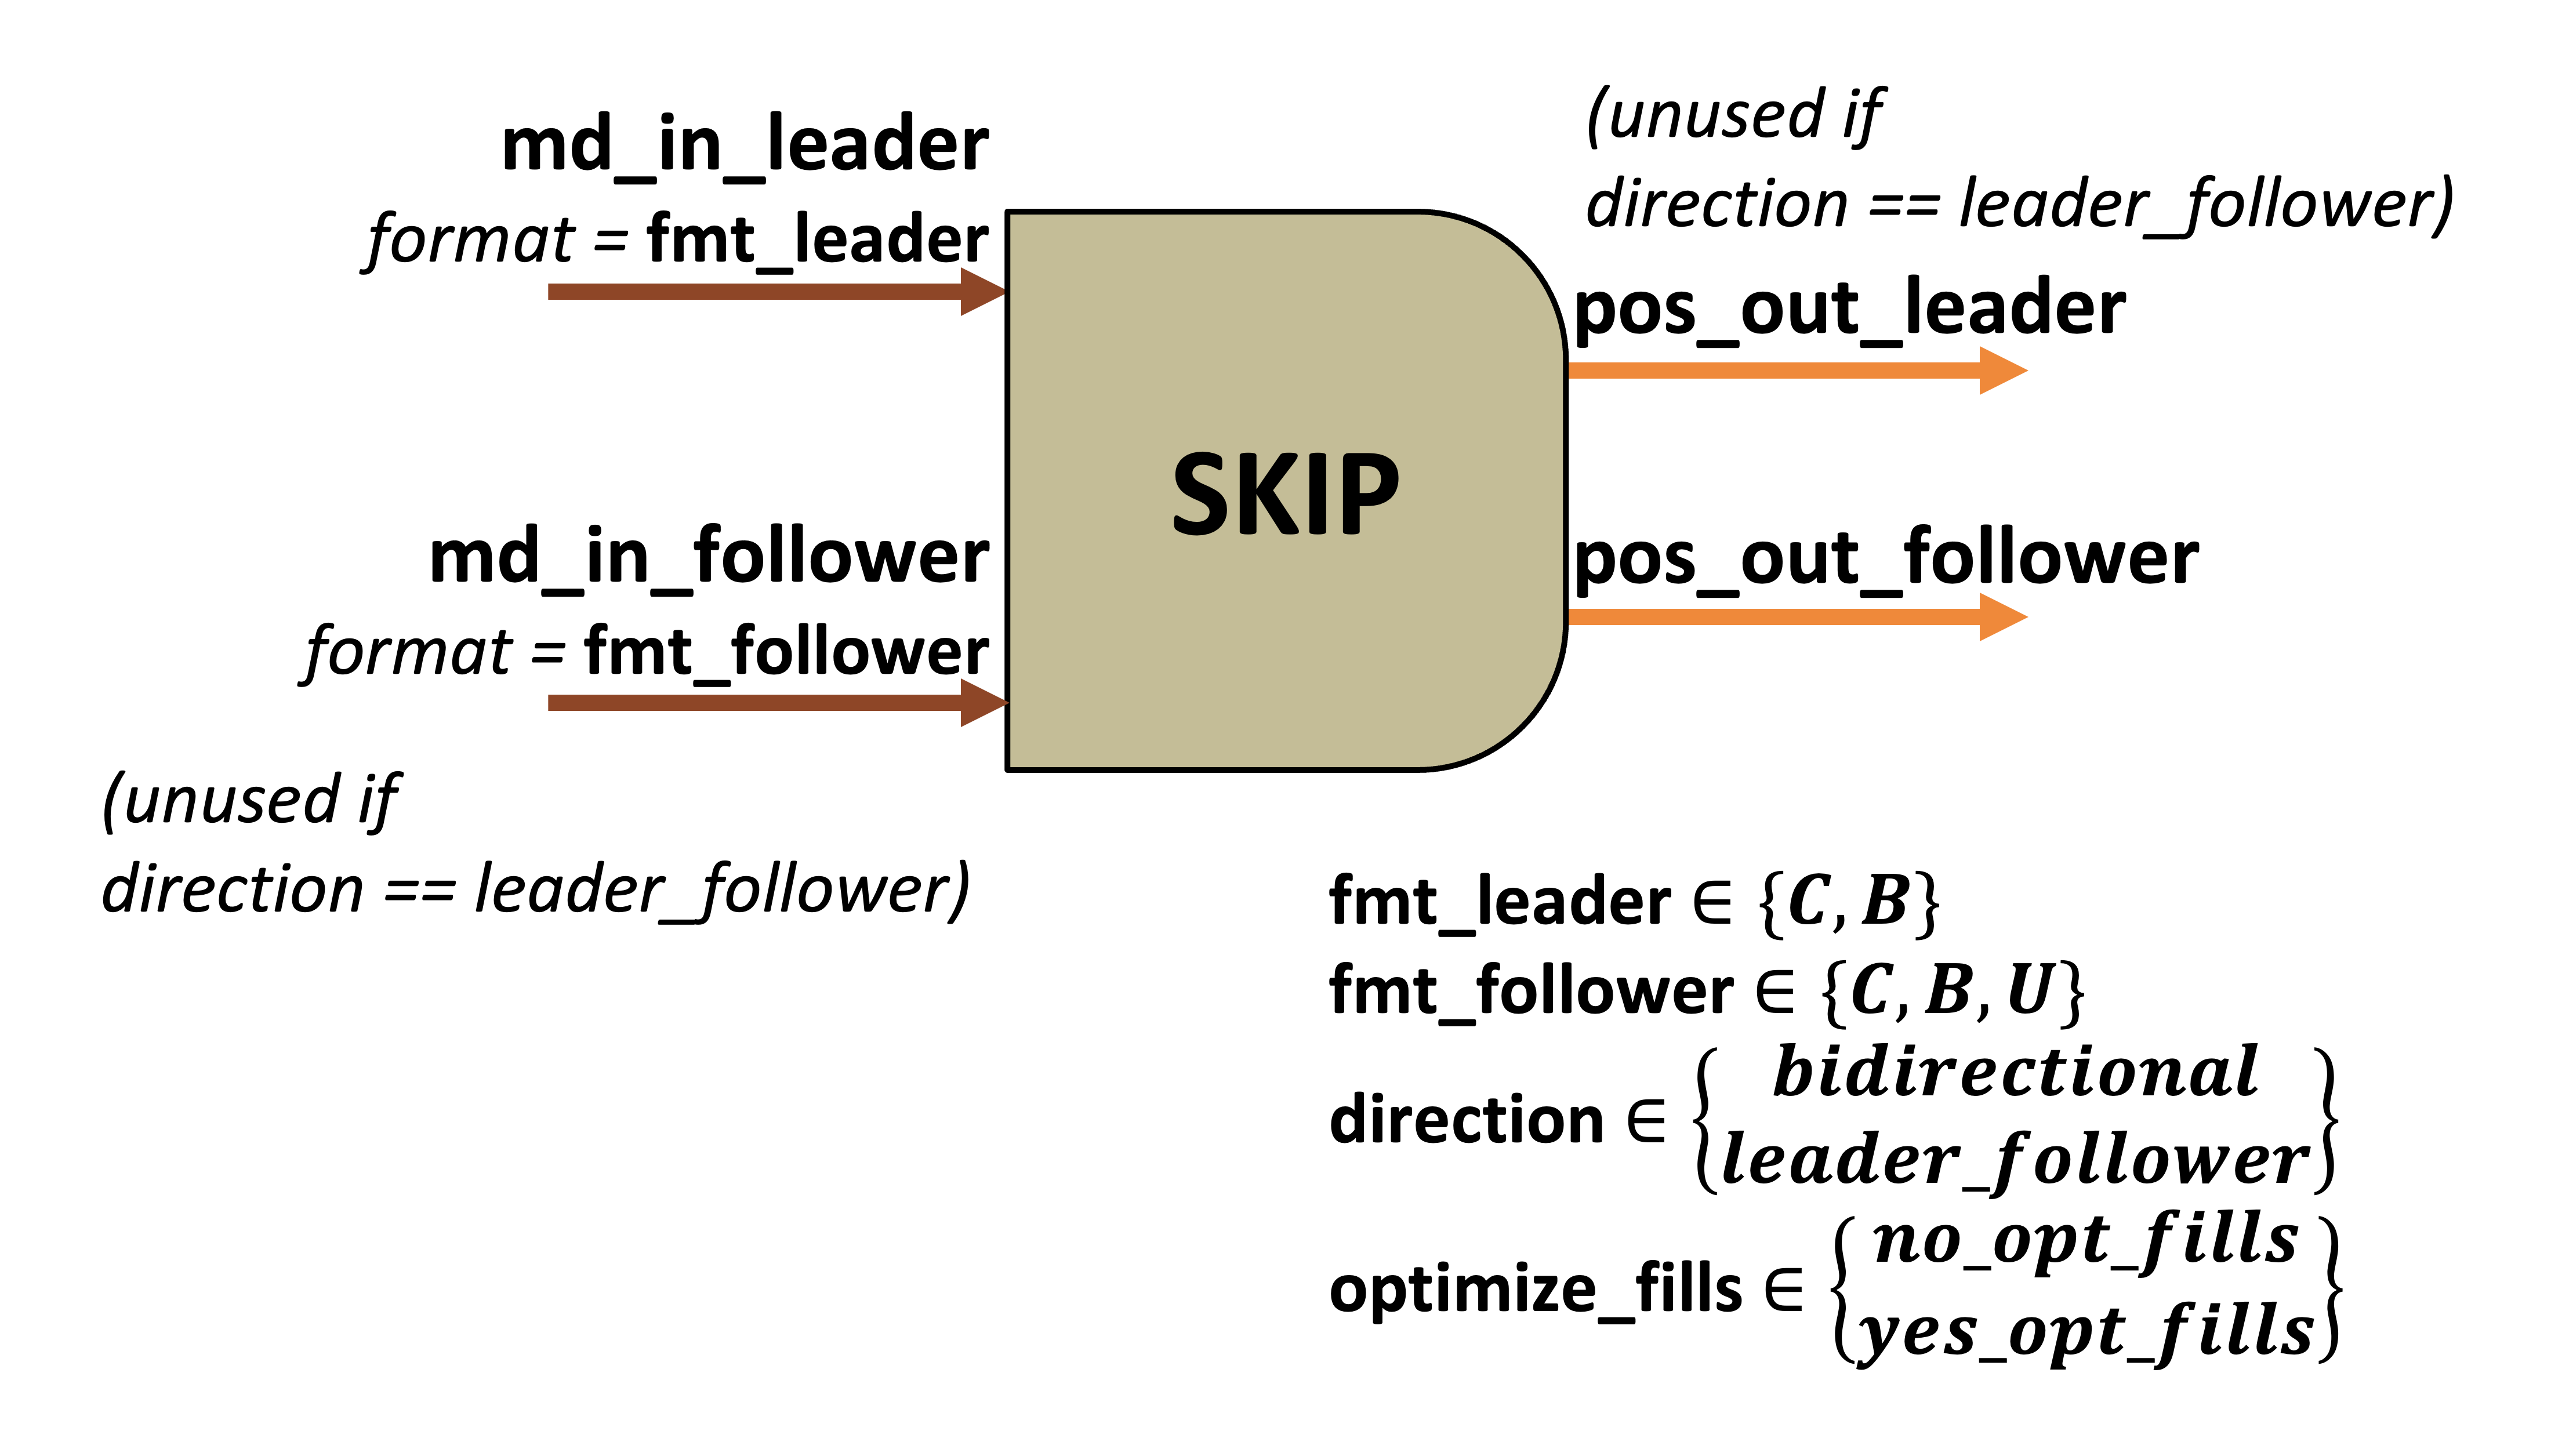
\includegraphics[width=0.95\textwidth]{figures/SKIP.png}
    \caption{Skipping microarchitecture compound component template.}
    \label{fig:SKIP}
\end{figure}

\subsubsection{Skipping microarchitecture specializations}

\begin{table}[ht]
\centering
\begin{tabular}{llll}
\toprule
 format\_leader   & format\_follower   & direction       & optimize\_fills   \\
\midrule
 C               & C                 & bidirectional   & no\_opt\_fills     \\
 B               & B                 & bidirectional   & no\_opt\_fills     \\
 C               & U                 & leader\_follower & no\_opt\_fills     \\
 C               & U                 & leader\_follower & yes\_opt\_fills    \\
\bottomrule
\end{tabular}
\caption{Specializations of skipping microarchitecture}
\label{tab:Skipping microarchitecture_specializations}
\end{table}

\begin{figure}[H]
    \centering
    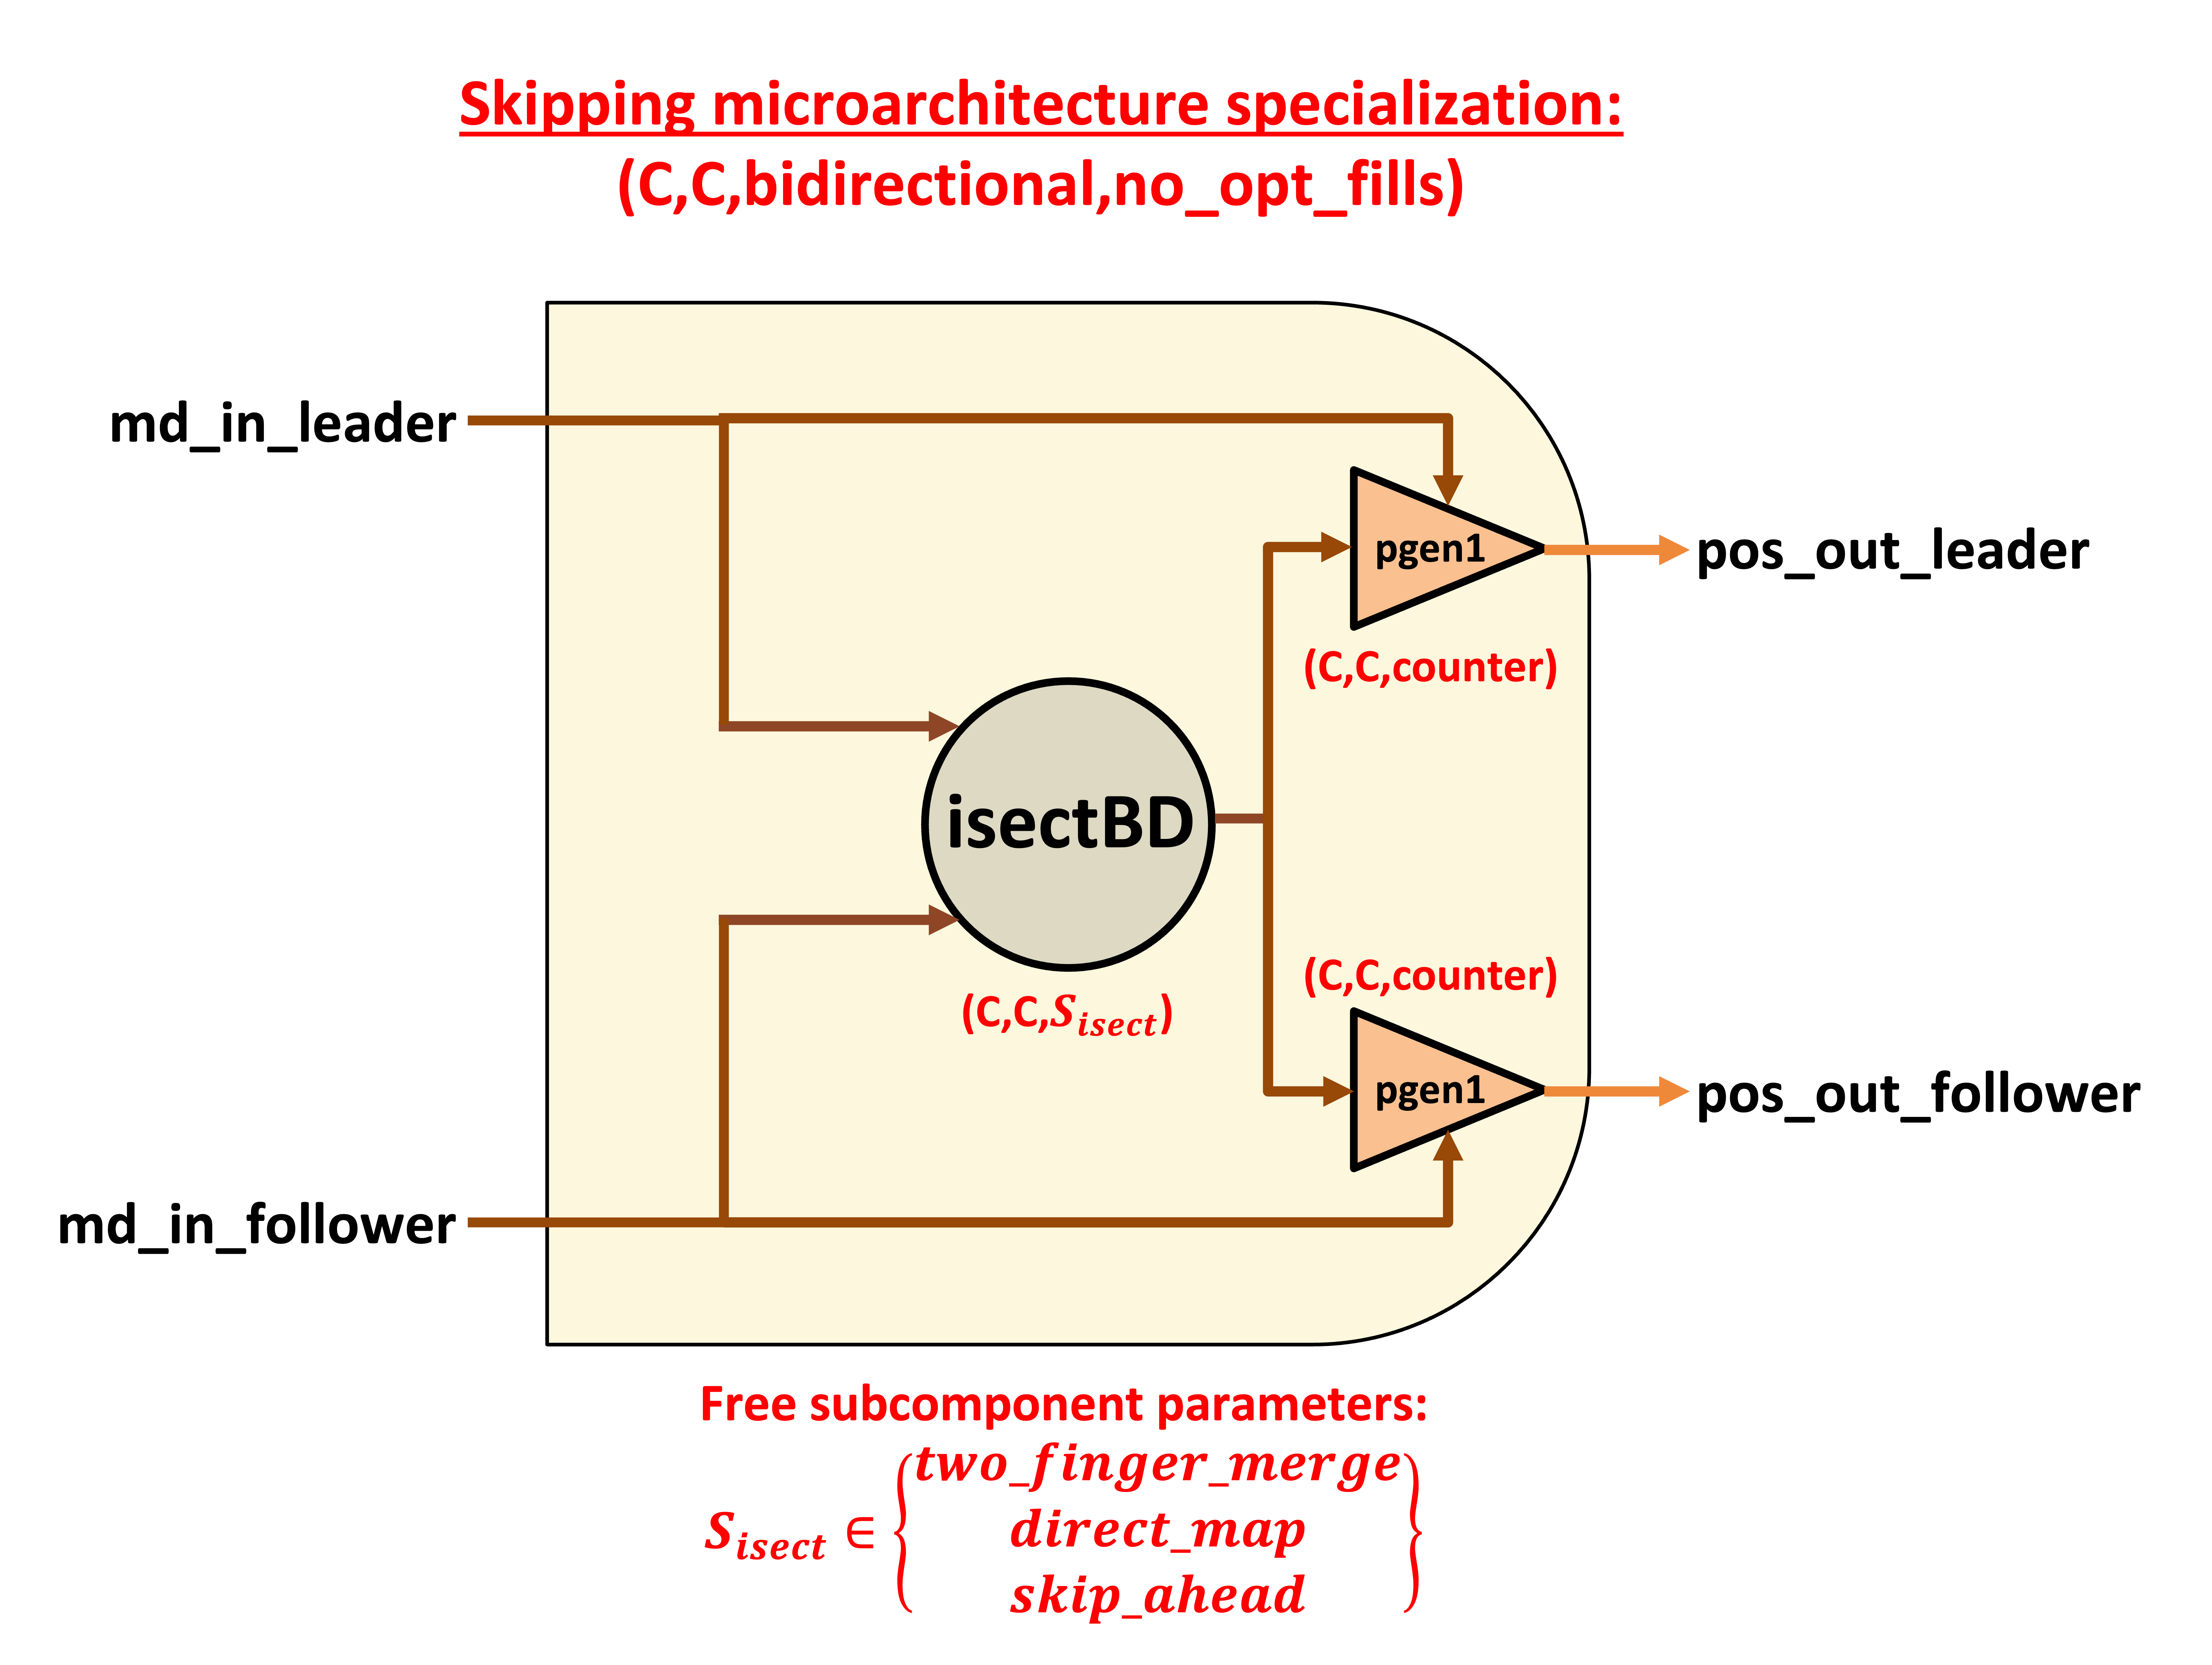
\includegraphics[width=0.95\textwidth]{figures/SKIP_C_C_bidirectional_no_opt_fills.png}
    \caption{Bidirectional coordinate-payload (C) skipping microarchitecture implementation topology (``ExTensor-like''\cite{extensor}.)}
    \label{fig:SKIP_C_C_bidirectional_no_opt_fills}
\end{figure}

\begin{figure}[H]
    \centering
    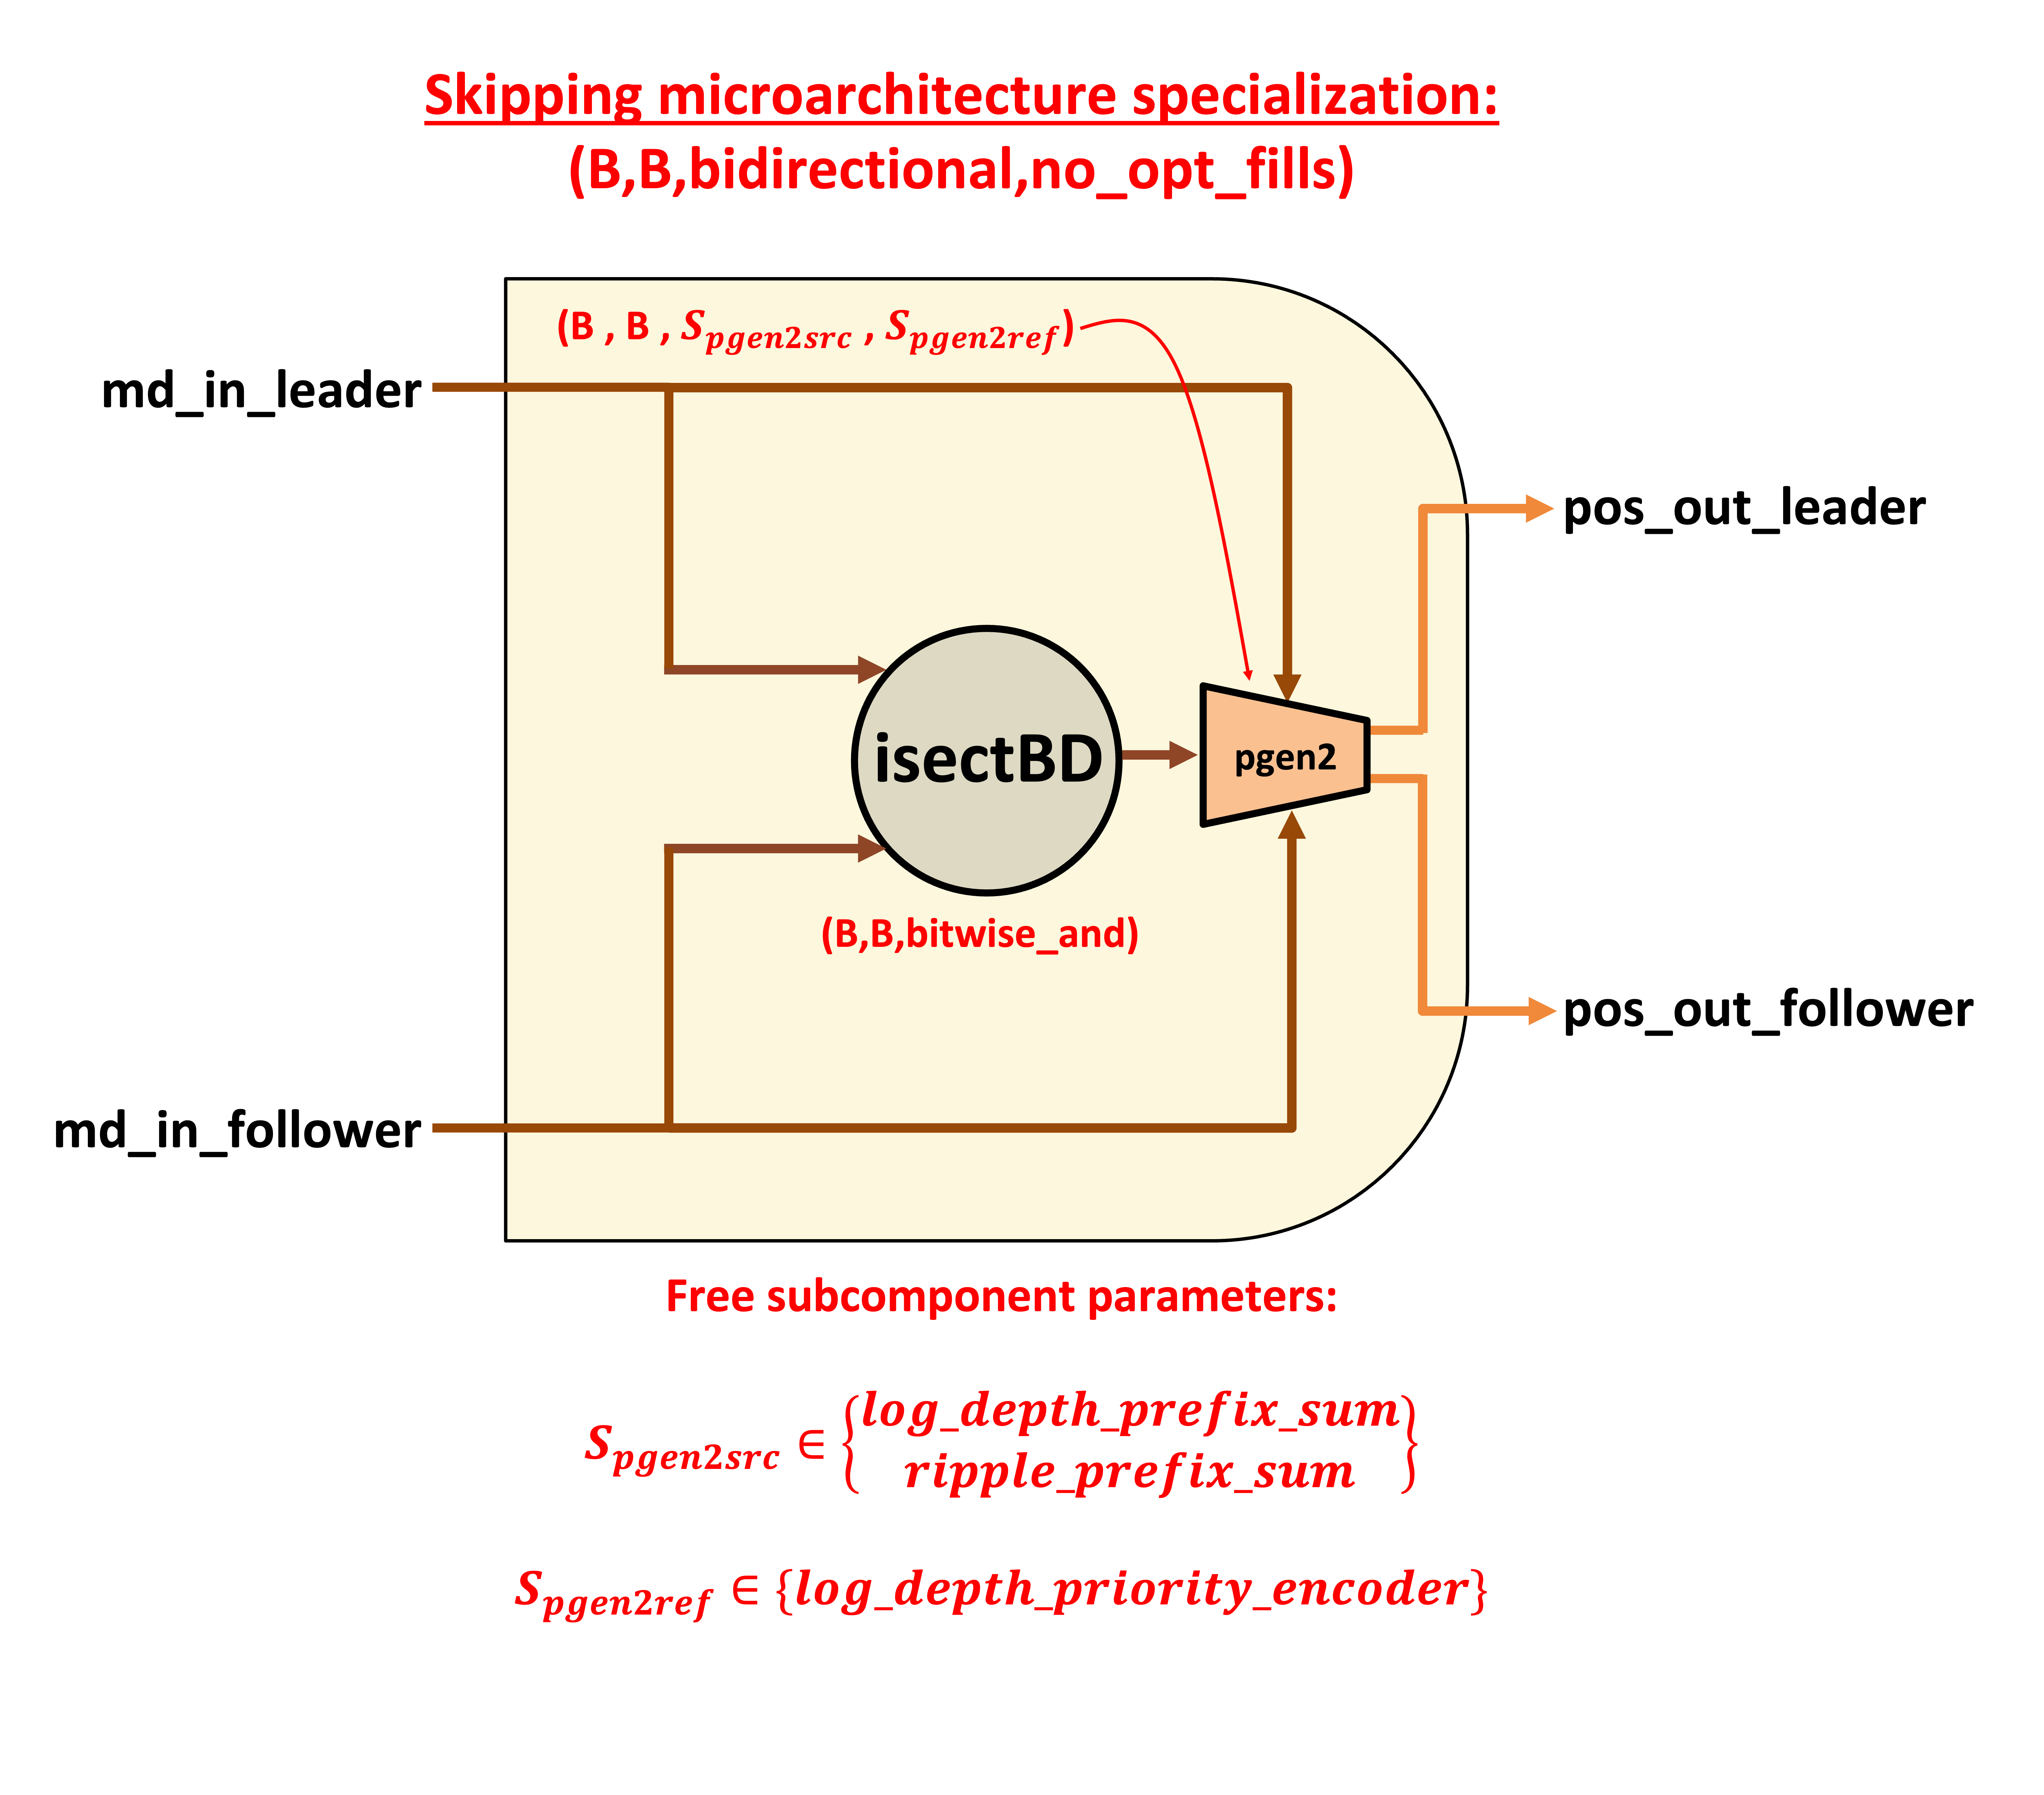
\includegraphics[width=0.95\textwidth]{figures/SKIP_B_B_bidirectional_no_opt_fills.png}
    \caption{Bidirectional bitmask (B) skipping microarchitecture implementation topology (``SparTen-like''\cite{sparten}.)}
    \label{fig:SKIP_B_B_bidirectional_no_opt_fills}
\end{figure}

\begin{figure}[H]
    \centering
    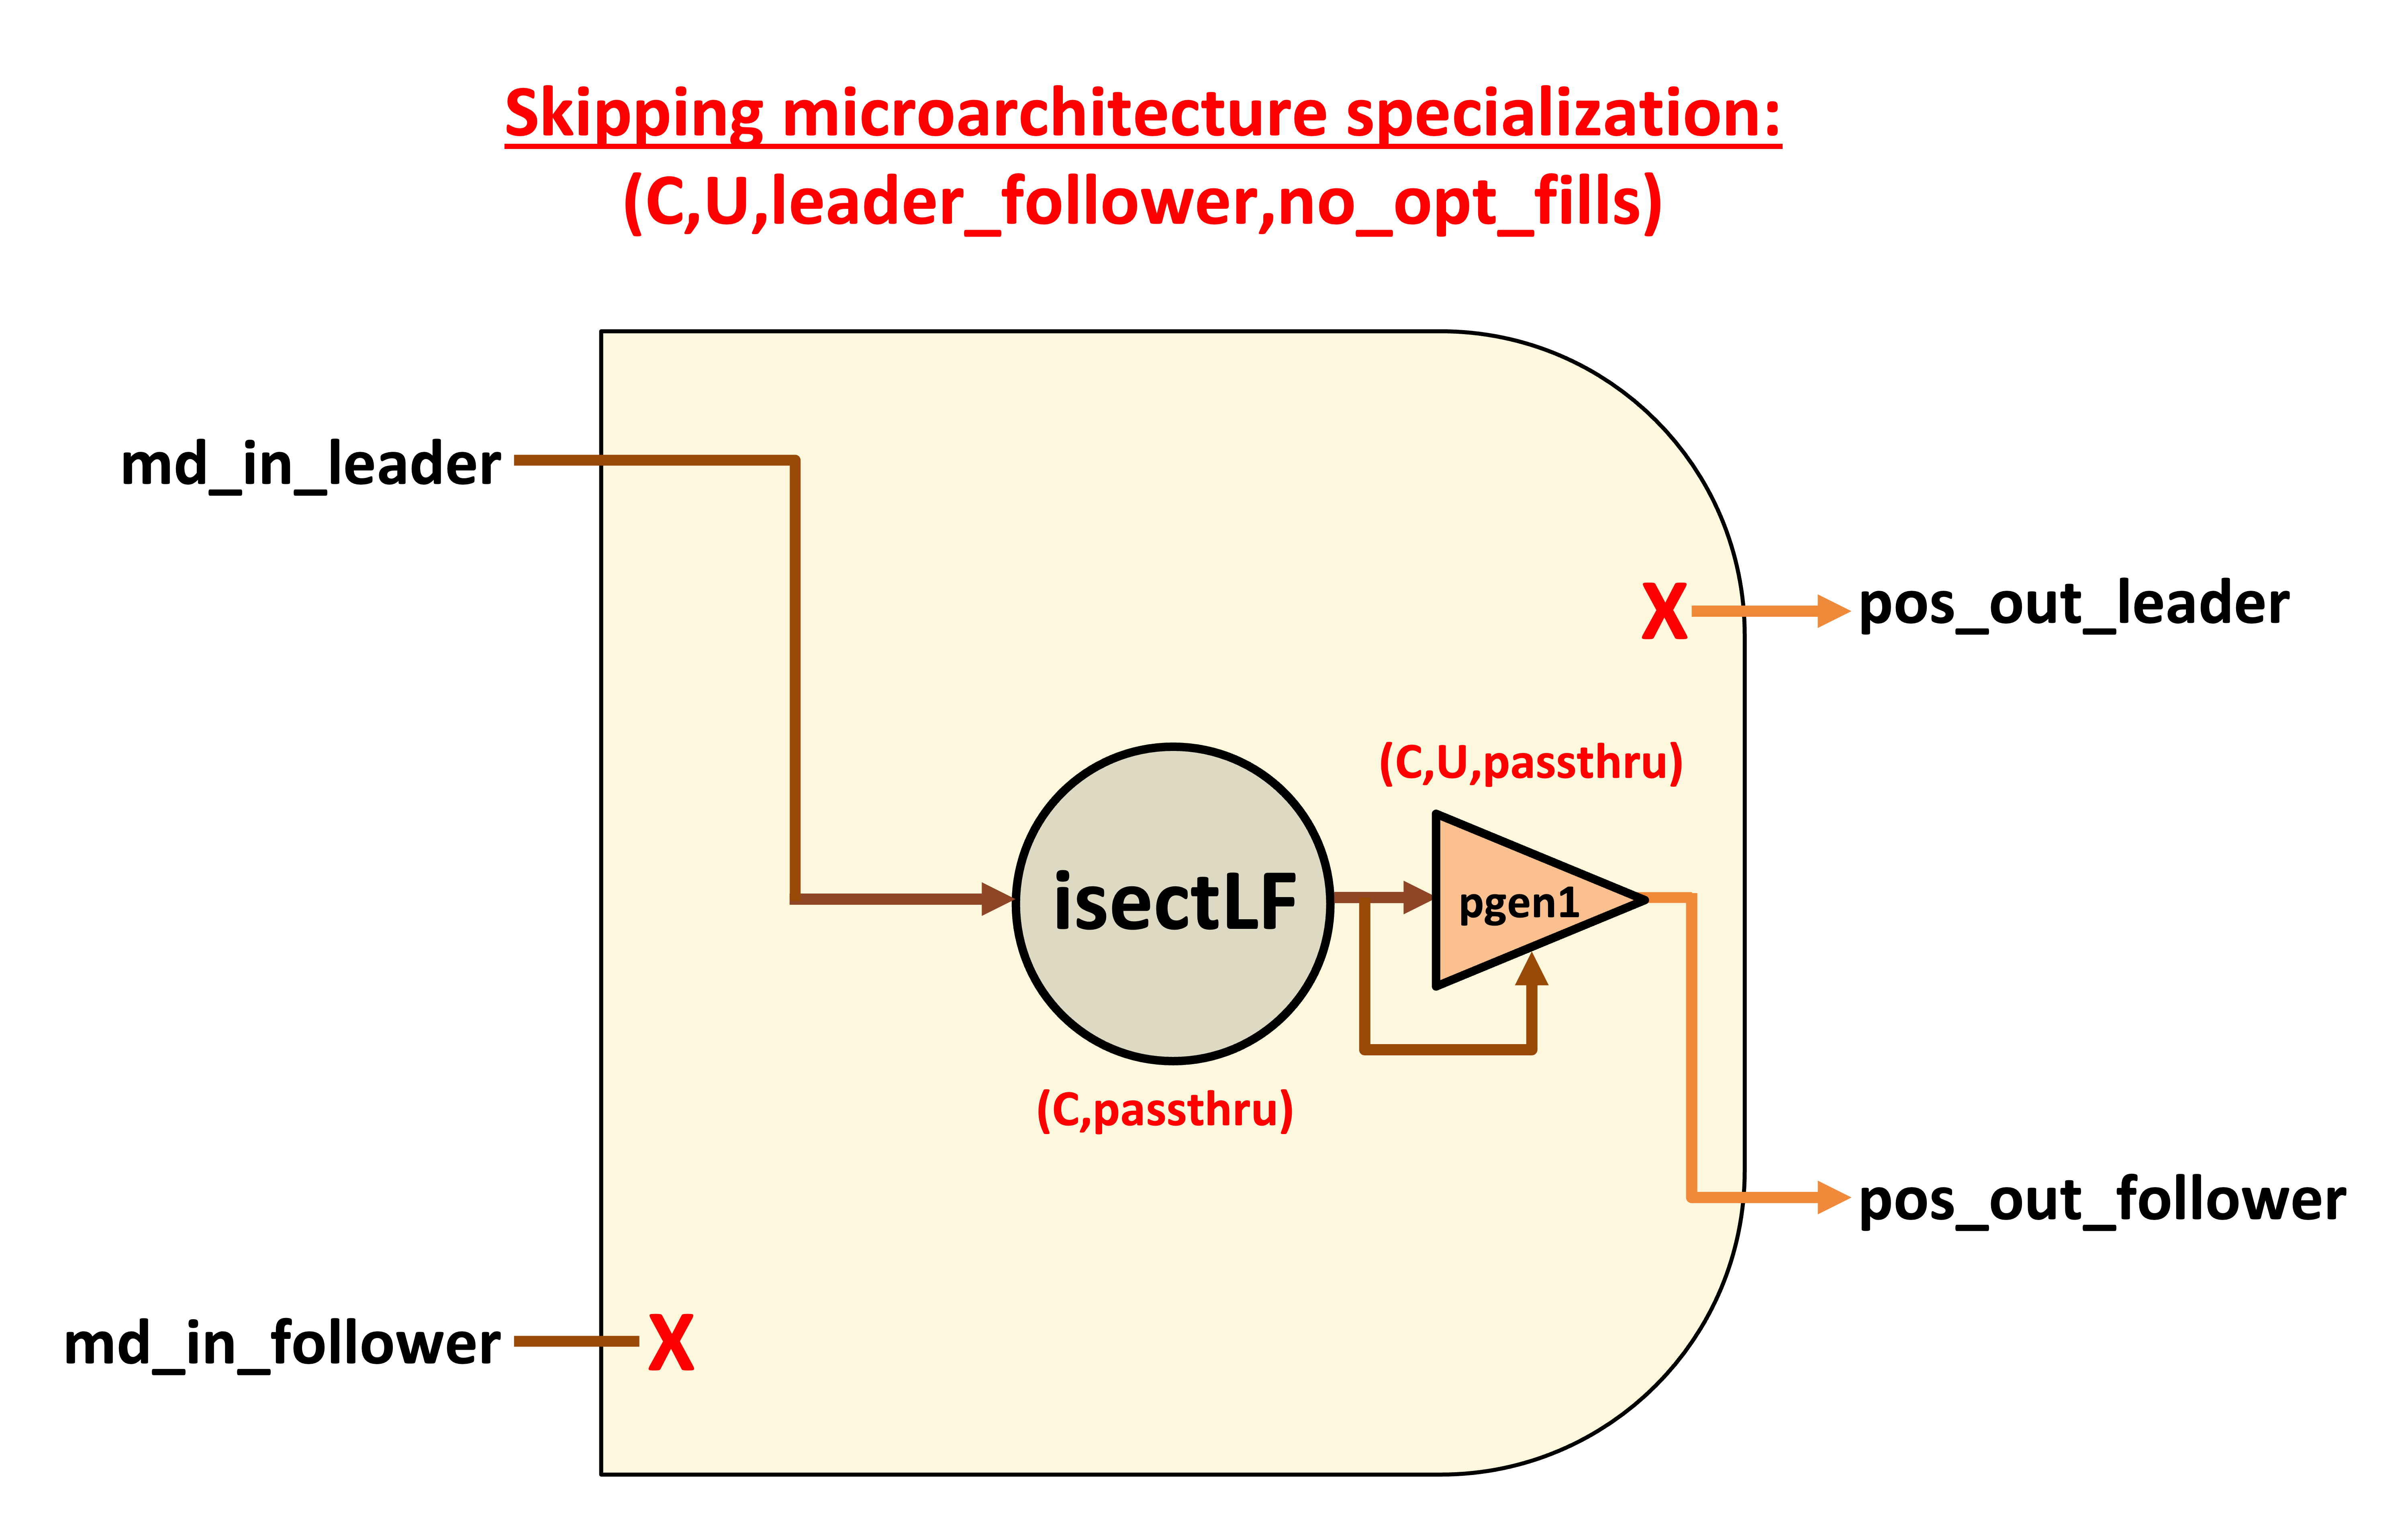
\includegraphics[width=0.95\textwidth]{figures/SKIP_C_U_leader_follower_no_opt_fills.png}
    \caption{Leader-follower coordinate-payload (C) to uncompressed offset-pair (U) skipping microarchitecture implementation topology, without fill optimization.}
    \label{fig:SKIP_C_U_leader_follower_no_opt_fills}
\end{figure}

\begin{figure}[H]
    \centering
    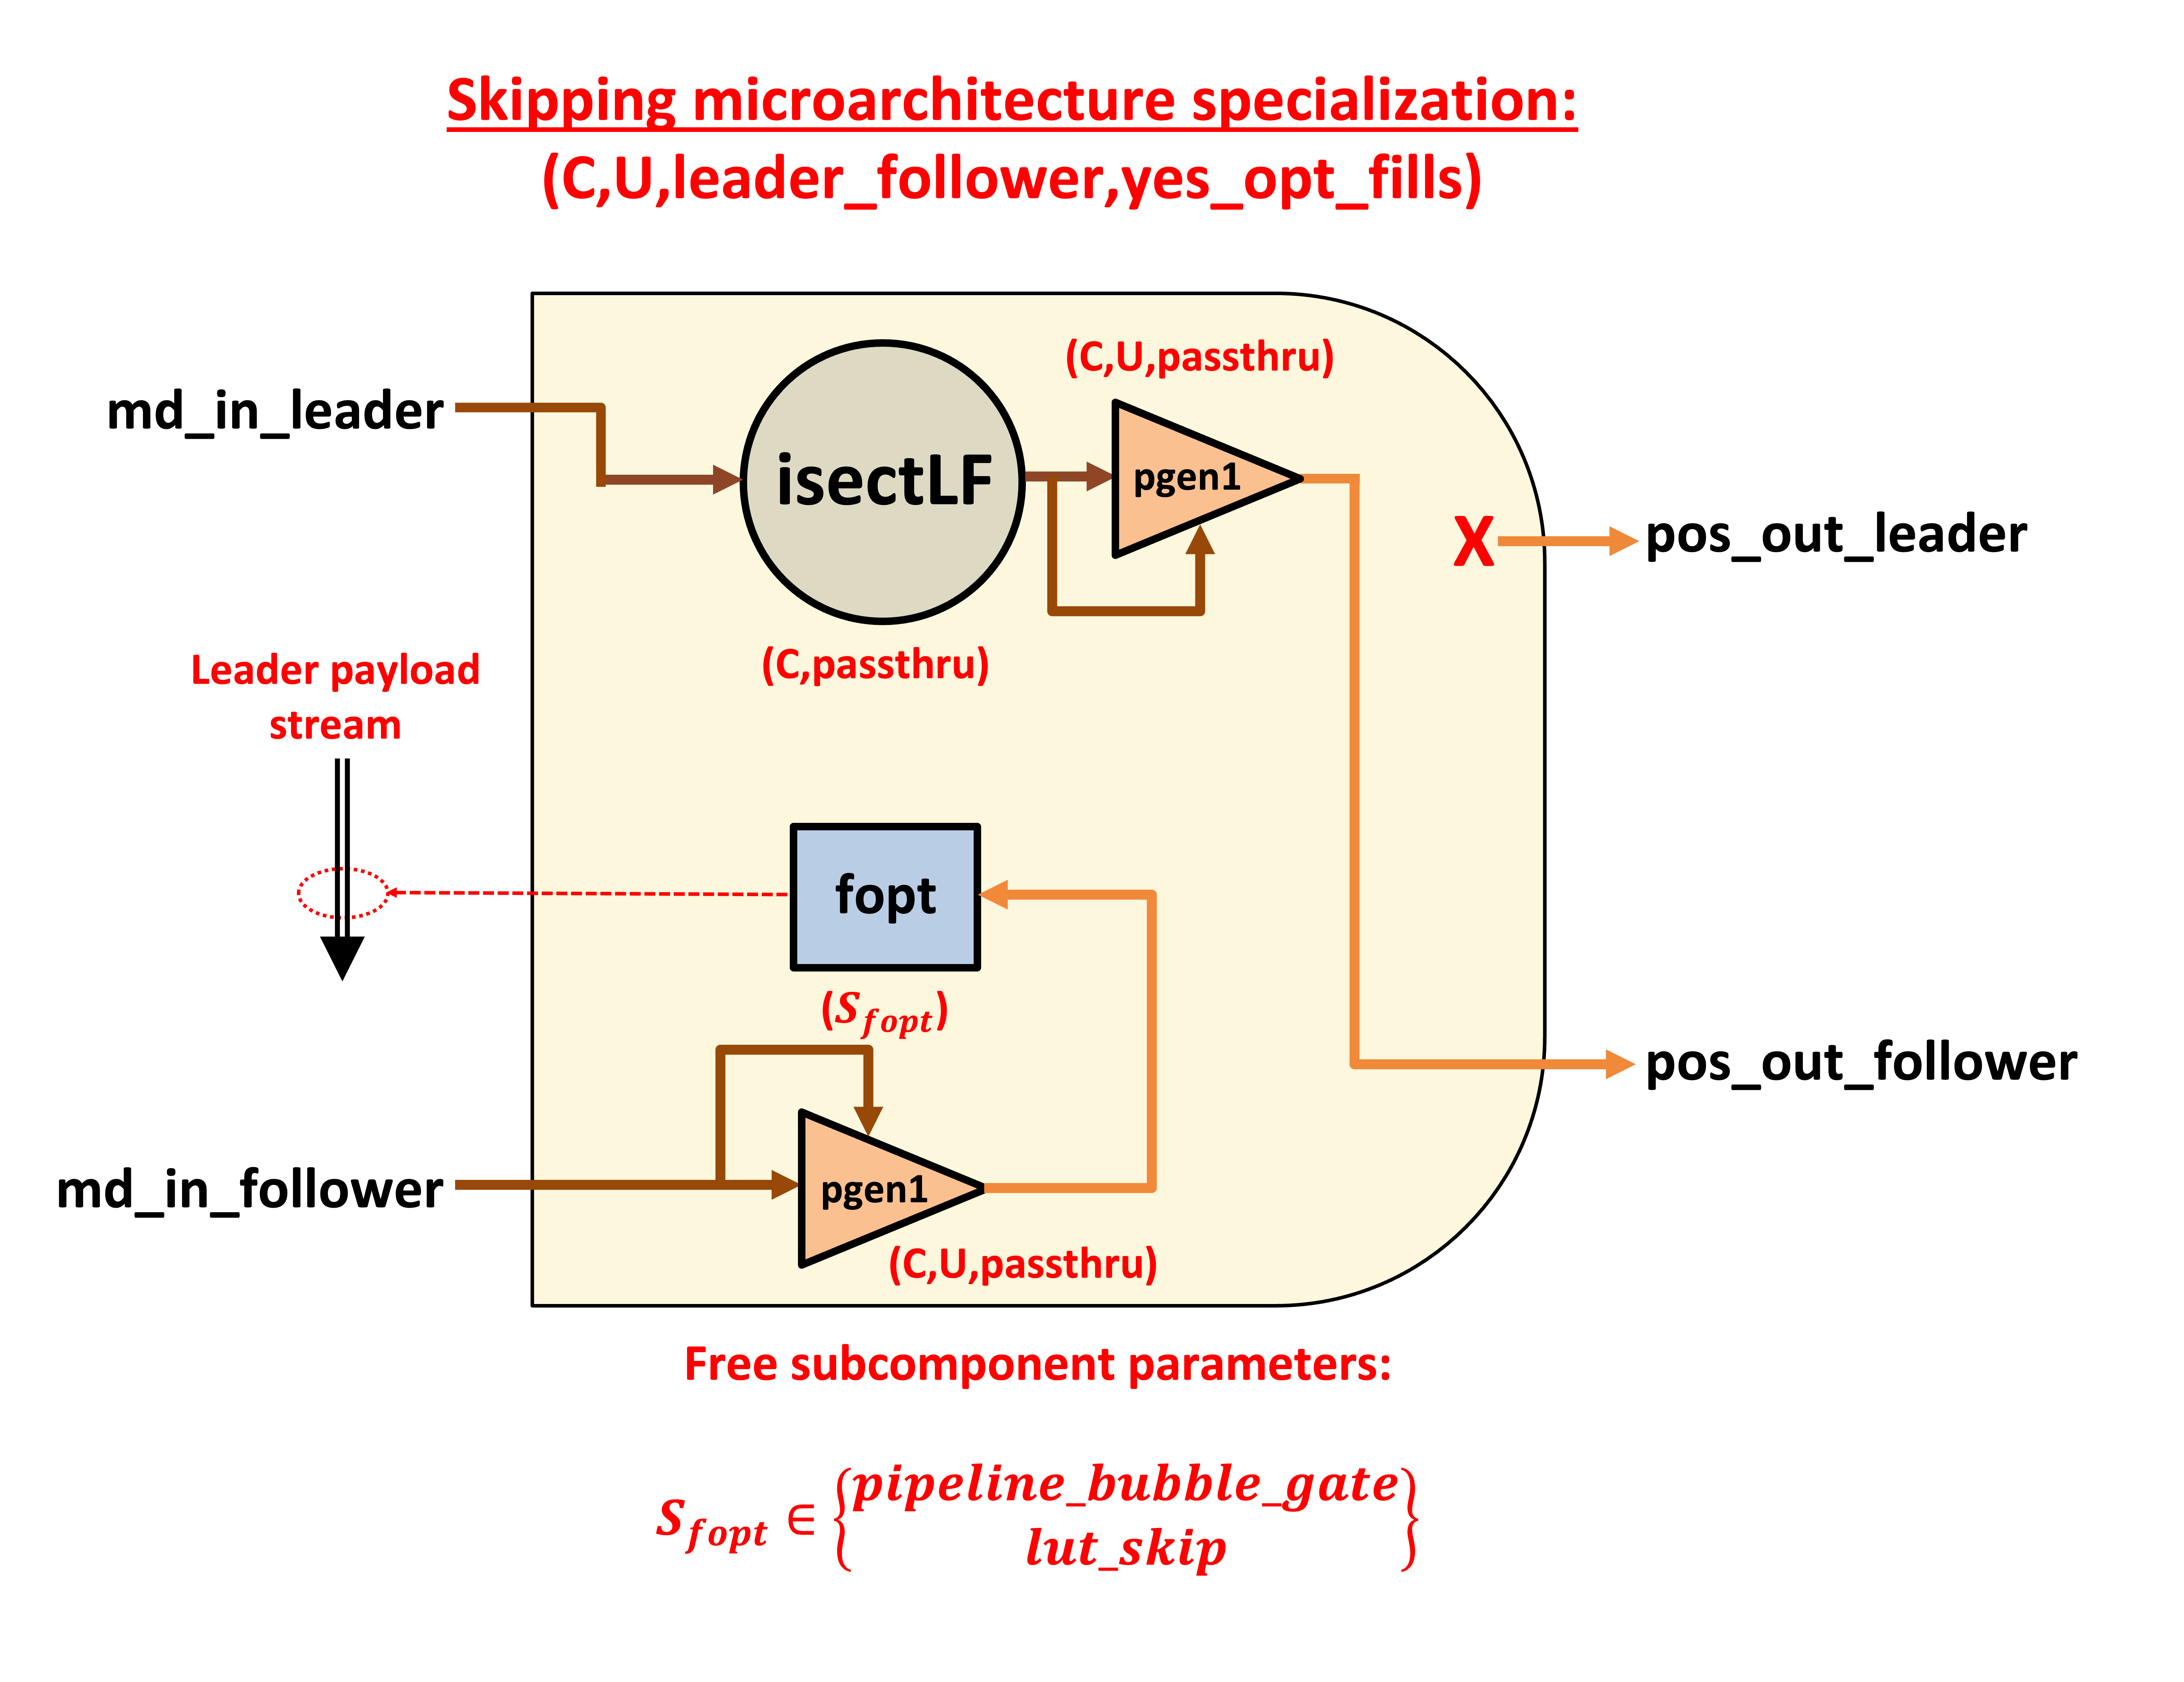
\includegraphics[width=0.95\textwidth]{figures/SKIP_C_U_leader_follower_yes_opt_fills.png}
    \caption{Leader-follower coordinate-payload (C) to uncompressed offset-pair (U) skipping microarchitecture implementation topology, with fill optimization (``Eyeriss-v2-like''\cite{eyerissv2}.)}
    \label{fig:SKIP_C_U_leader_follower_yes_opt_fills}
\end{figure}

\section{SAF concretization}
\label{chapter:saf_concretization}